\section{Control Genomes}
\begin{figure}
    \centering
    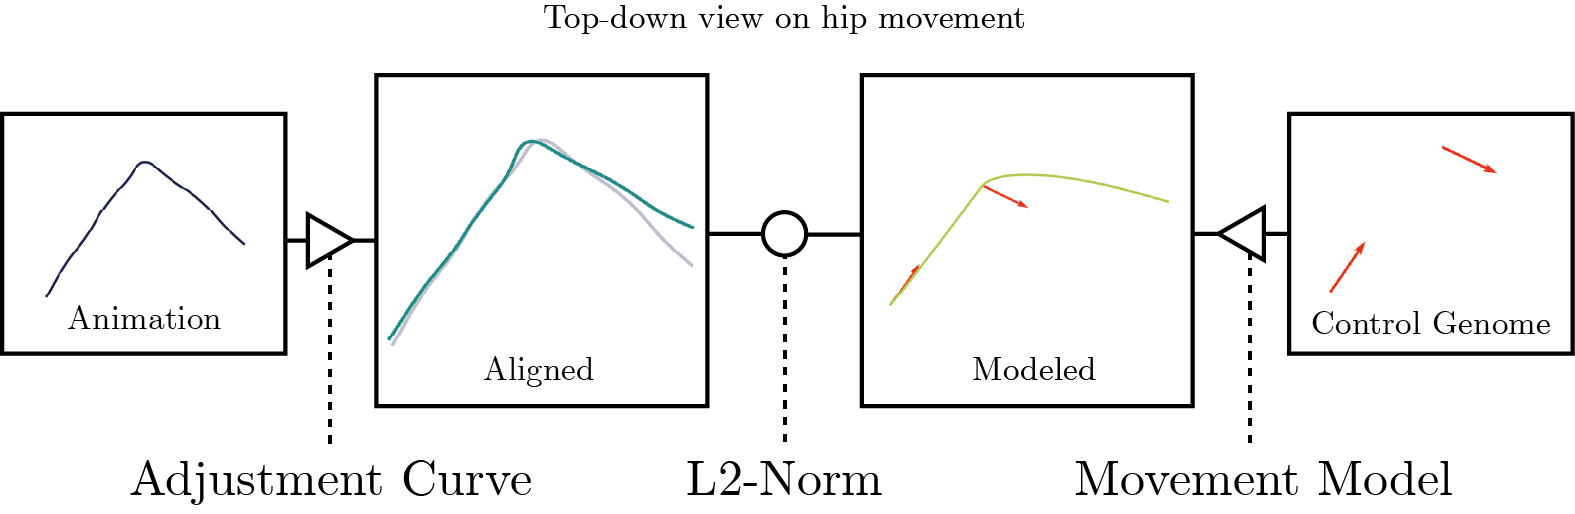
\includegraphics[width=1\columnwidth]{img/overview}
    \caption{System overviews}
    \label{fig:movement:overview}
\end{figure}
Human movement is a complex interplay between intentions within the brain and the physical environment. The thought to 'walk-forward' triggers an array of intractable optimizations. A movement model is similar when high level gamepad input is mapped to low level control signals. We notice that if no restrictions are imposed to the granularity of the high level signal, it can in the limit approach the low level signal we wish to model. In this perspective the modeling task is ill-posed, and we suggest control genomes as a method to regularize the task by formalizing the complexity of the high level input signal.   

In the following we will introduce an end-to-end method for synchronization between a movement model and a set of reference animations using control genomes. There are 4 main parts to the method. 
\begin{itemize}
    \item \textbf{Control genomes} extracted from animations.
    \item \textbf{Movement model} that generates a movement given Control Genomes.
    \item \textbf{Trajectory estimation} and alignment of reference animations to avoid modeling unwanted details. 
    \item \textbf{Optimization procedure} to fit exposed parameters of all the above systems to minimize the difference between the movement model and the reference animation.
\end{itemize}
Figure \ref{fig:movement:overview} illustrates the definitions and concepts of a movement model.

\subsection{Control Genomes}
We define Control Genomes as signals that can generate movement. They are a combination of intentions and enough contextual state to follow the Markov principle. As an example a position, direction and time is a control genome for a straight walk. Conversely a straight walk contains a latent control genome (position, direction, time). Under this naive framework we quickly realize that multiple straight walks could be associated with a single control genome. We further impose the constraint that control genomes must disambiguate movement. That means a unique control genome maps to a unique movement. In our simple example we might resolve conflicts by adding a style parameter and assign values such as 'brisk walk' or 'dragging feet' to our control genomes. 

Control genomes can have a direct counter part in the host application such as user input through a game controller or navigational path from an AI system, and therefore can also be viewed as tasks that are carried out by the animations, for instance turn to right. In general we want the control genomes to be of minimal size, since in the limit we could have the animation itself as the control genome. We say that a genome is in \textit{reduced} and \textit{segmented} form if it contains no repetitions and removal of information would break either the Markov property of the disambiguation constraint. 

\begin{figure}
    \centering
    \kenny{I dislike the style of the figure. It stands out compared to the better visual quality papers. A coherent style everywhere is better, if style looks messy then it colors reviewers opinion of the work.\\}    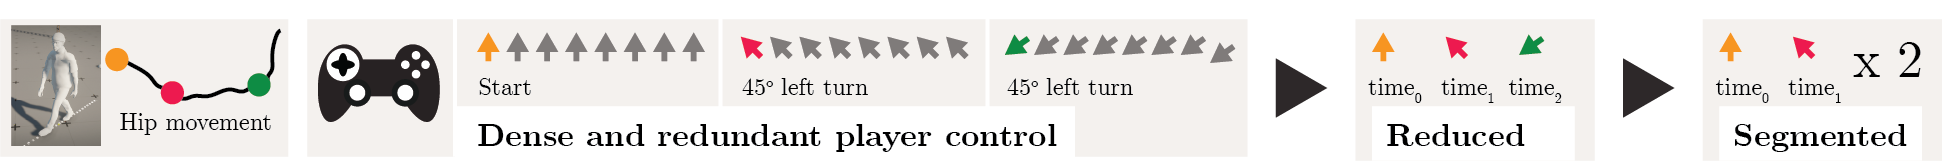
\includegraphics[width=1\columnwidth]{img/controlgenome.png}
    \caption{Control Genome.}
    \label{fig:control:genome}
\end{figure}

Figure \ref{fig:control:genome} shows an example where an animation has been assigned a control genome. Each frame is annotated with a 2D-control direction corresponding to stick input from a game controller. A dense and redundant control genome contains the entire skeletal animation as well as the annotated directions. The animation has two similar right turns so we get a single segmented control genome by splitting the redundant genome in two identical parts. We then trim all unnecessary information from the genome to get the reduced form which only contain a starting position and two direction offset in time. This last step assumes that we are capable of regenerating the animation from the reduced genome using a model we will refer to as a \textit{Movement Model}. A Control Genome paired with a Movement Model describes an animation exactly when the Movement Model can regenerate the Animation from the Control Genome.  In practice it is not possible to develop accurate generative or predictive models for human movement. So we will allow our animations to undergo non destructive transformation such as smoothing and path adjustment, and only expect our model to regenerate a fraction of the complete signal, such as the trajectory. 

We will now proceed to a formalized description of control genomes. The input to our method is an annotated animation. Let $\anim^{\dimas,\dimaa}_\dimat$ denote $\dimat$ frames of animation of a skeleton with $\dimas$ degrees of freedom, where each frame is given an $\dimaa$-dimensional annotation. 

We assume there exist an automated or manual Retrieve-and-Collapse function, $\reco$,  that extracts all reduced and segmented control genomes present in the animation and for each maintains a pairing to all $k$ corresponding un-annotated segments of the source animation. That is $\reco$ converts a source animation into an associate map, $\lut$, that uses genomes as keys and un-annotated segments of source animation as values. We may write $\reco(\anim^{\dimas,\dimaa}_\dimat) \rightarrow \lut$. Now given the $i\th$ control genome of dimension $\dimg$ we have
\begin{equation}
 \lut(\genome^g_i) \rightarrow \left\{\anim^{\dimas,\dimaa}_{\dimae_0},\ldots,\anim^{\dimas,\dimaa}_{\dimae_k}\right\}   \,,
\end{equation}
where $\dimae\ll\dimat$ refers to a segment of the full animation and $k$ is the number of segments matched to the $i\th$ control genome.

We define two parametric projections, $\model$ and $\edit$, to a shared $\dimes$-dimensional space, $\mathcal{R}^{\dimes}$, as follows
\begin{align}
\model(\paramm,\genome_i^{\dimg}) 
&\rightarrow 
\mathcal{R}^{\dimes}    \,,
\\
\edit(\parame,\anim_{\dimae}^{\dimas,\dimaa})
&\rightarrow
\mathcal{R}^{\dimes} \,,
\end{align}
where $\paramm$ and $\parame$ are free parameters to be optimized for later. We call $\mathcal{R}^{\dimes}$ an evaluation space and it will usually have a natural counterpart in the application such as the trajectory (position and orientation of character over time).
u
Intuitively $\model$ is a Movement Model capable of generating movement or more accurately an evaluation space representation from the control genomes. $\edit$ corresponds to the adjustment we allow our animations to undergo, such a smoothing or more advanced manipulation. The optimal parameters for a single control genome are found as the minimization of the L2-norm.
\begin{subequations}
\begin{align}
    \gnorm(\paramm,\parame,\genome_i)
    &\equiv
    \sum_{\anim_k\in\lut(\genome_i)}
    {
        \frac{1}{2}
        |\model(\paramm,\genome_i)
        -
        \edit(\parame\anim_k)|^2
    }
    \label{eq:optim:single}
    \\
    \paramm^*,\parame^*
    &\equiv \arg\min_{\paramm,\parame}
    {
        \gnorm(\paramm,\parame,\genome_i)
    }
\end{align}
\end{subequations}
When we want constant parameters across the fitting of multiple control genomes an additional term is added to the minimization. 
\begin{equation}
    \vec{\paramm^*},\vec{\parame^*}
    \equiv 
    \arg\min_{\paramm,\parame}
    \left(
        \sum_{\genome_i}
        \gnorm(\paramm^i,\parame^i,\genome_i)
    \right)
    +
    VAR(\vec{\paramm},\vec{\parame})
\end{equation}
Where $\vec{\paramm^*},\vec{\parame^*}$ is the full set of parameters and $\paramm^i,\parame^i$ are the parameters fitted to $\genome_i$.

\subsection{Movement Model}
\begin{figure*}
    \centering
    \kenny{I dislike the style of the figure. It stands out compared to the better visual quality papers. A coherent style everywhere is better, if style looks messy then it colors reviewers opinion of the work.\\}    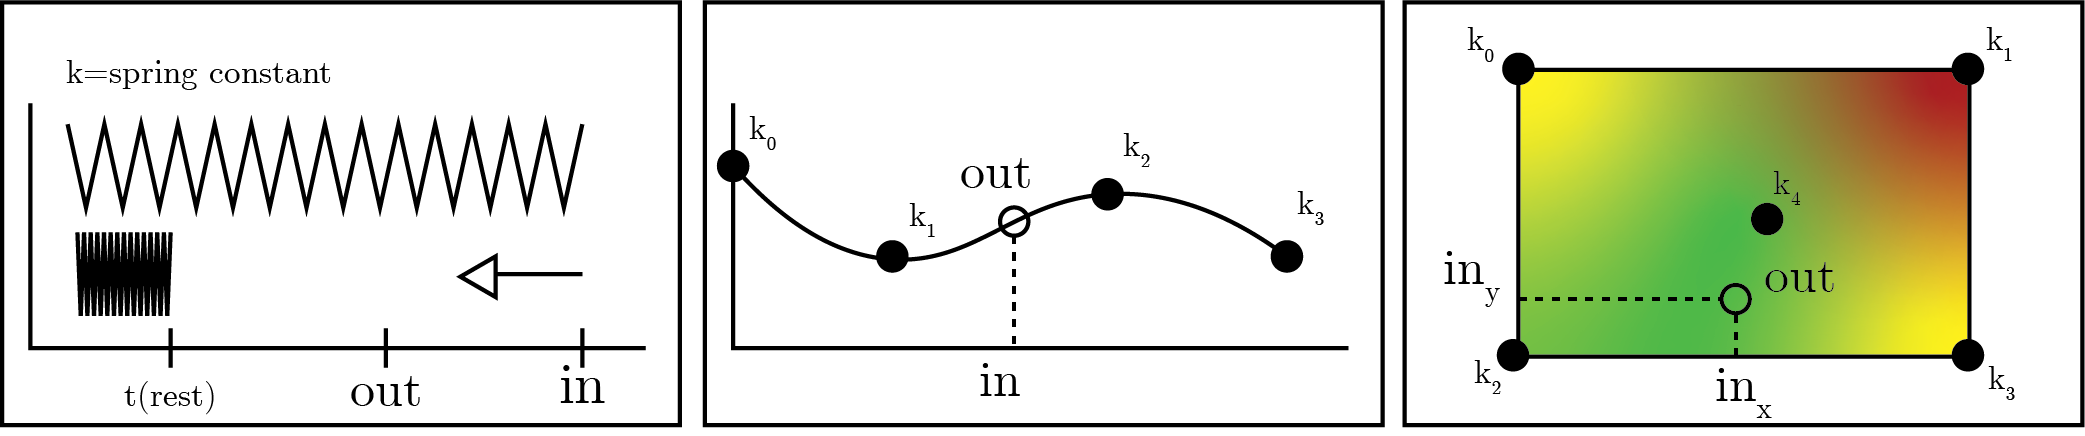
\includegraphics[width=0.75\linewidth]{img/model_primitives}
    \caption{Planning primitives. K values indicate parameters subject to optimization.\kenny{Please state what reader should learn from this figure.}}
    \label{fig:movement:prims}
\end{figure*}
In this section we will describe how movement can be generated from Control Genomes using a Movement Model. Without loss of generality, we will examine plane locomotion and limit the output of the model to trajectories, which is time series of connected positions and facing directions. 
Conceptually there are no limitations on the complexity of the models we chose. Dense neural networks [ref] or muscle based physical simulations [ref] are capable of even generating full body locomotion. However we would like a model that exposes easily and exactly tweakable parameters to the game designers and animators. In many game scenarios micro timings and the 'feel' of the character movement are core parts of the user experience. Accordingly we need descriptive models, that can still be transparently manipulated by the artists. 

We use the trajectory as evaluation space with $\pos$ and $\facing$ as the 2D plane position and 1D rotation around the up-axis over $t$ frames. Hence we have dimension $\dimes = 3 t$ for our evaluation space,
\begin{align}
\mathcal{R}^{3 t} 
\equiv 
\left\{
    \pos_0,\facing_0,
    \ldots,
    \pos_{t-1},\facing_{t-1}
    \right\}
\end{align}
We construct Control Genomes as an initial state followed by a sequence of movement characteristics we would like to achieve. Player input is supplied through standard gamepad control using stick direction and button presses with $\left\{ \controlmove_d, \controlface_d \right\}$ representing the desired facing and movement directions at time $d$. Further parameters can be added to support different movement styles and are controlled with button presses. The simplest genome would contain an initial state and a single control input: $\genome^5 \equiv \left\{ \pos_0,\facing_0,\controlmove,\facing^c \right\}$. Additional data can be added to the Control Genomes either by expanding the data contained in the initial state, by adding additional types of control values or by providing a time series of control values which are then treated as a step curve. A non-parametric Movement Model maps from Control Genome to evaluation space
\begin{equation}
    \model(\goals^5)
    \rightarrow
    \underbrace{
    \left\{
    \pos_0^m,\facing_0^m,\ldots,\pos_{t-1}^m,\facing_{t-1}^m\right\}
    }_{\in \mathcal{R}^{3t}}
    \,,
\end{equation}
and is easily described as recursive updates to the initial genome state. If the state is expanded with additional values those are also integrated by the Model. 
We may write this in an abstract notation by using a generic update function $\mathcal{U}$ as follows,
\begin{subequations}
\begin{align}
    \left\{
    \pos_d^m,\facing_d^m
    \right\}
    &\leftarrow
    \left\{
    \pos_0,\facing_0    
    \right\},&d=0
    \\
    \left\{
    \pos_{d+1}^m,\facing_{d+1}^m
    \right\}
    &\leftarrow
    \mathcal{U}
    (
    \left\{
    \pos_d^m,\facing_d^m,
    \controlmove,
    \controlface,
    \dt
    \right\}
    )
    \label{eq:move:update},&d>0
\end{align}
\end{subequations}
The update acts as motion planning by controlling how the current state transitions towards a new state as defined by the Control Genome. We impose a restraint to model this transition process according to the characteristics of the reference animation, by parameterising $\model$ and optimizing using the objective function \eqref{eq:optim:single}. 

It is by no means trivial to construct a general $\model$ even for plane locomotion. Instead we opt for a modular approach where the planning function in \eqref{eq:move:update} is a composition of planning primitives that can be arranged for different levels of expressiveness. Each primitive exposes a set of adjustable parameters and performs input to output mapping using various interpolation methods. In the limit the compositions could approximate full neural networks, but should be kept simple enough for human manipulation of each parameter while maintaining the capability to model the movement in the reference animations.     

Fig. \ref{fig:movement:prims} illustrates the 3 planning primitives we use to model plane locomotion, where $\theta^d$ indicate $d$-dimensional values that can be optimized. Our primitives in this work are:

\begin{itemize}
\item{\bf Spring primitive:} We use a critically damped spring primitive that depends only on one parameter $\theta^1 \in \Re_+$. Given input $x \in \Re$ we can write the primitive mathematically as a mapping to the output $y \in \Re$ as $y \leftarrow \spring{( x , \dot{x}, \theta^1, x^\prime, \dt)}$. Here $\theta^1$ exposes a spring coefficient used to control the drag of the input variable towards the target $x^\prime$. It is essentially a time-integration over $\dt$ of a spring force with initial conditions $x$ and $\dot{x}$.

\item{\bf 1D interpolation:} The 1D-Map interpolation map uses $\theta^d$ with $d>1$ data-values to find the interpolated value $y \in \Re$ of input $x \in \Re$. We write this as  $y \leftarrow \mapo(x,\theta^{d})$. With out loss of generality we choose to use spline interpolation over 4 knots.

\item{\bf 2D interpolation:} The 2D-Map interpolation is similarly defined. Except it maps input $x_0,x_1 \in \Re$ to output $y_0,y_1 \in \Re$ $(y_0,y_1) \leftarrow \mapt( (x_0, x_1),\theta^{d})$. In our implementation we use barycentric coordinates to interpolate polygon knots according to a 2D grid position given as input.    
\end{itemize}

As an example we propose a Movement Model for plane locomotion typical for 3rd person computer games  \kenny{how can you prove it is typical? any cites for this?} that strikes a compromise between simplicity and expressiveness. We use the convention that an $i$ superscript refers to intermediary values used temporarily during the model update \kenny{The superscript notation really clutters the math in my opinion. Perhaps using hat or tilde might be simpler layout wise?}. 
%
First for getting control of speed, move direction and angular speed ie. rate of change of the movement direction the position and facing information contained in the Control Genome state is augmented with derived values $\speed_0, \move_0, \angularspeed_0$. 
%
Compared to $\genome^{5}$ the expanded Control Genome looks like this,
\begin{subequations}
\begin{align}
    \genome^{8} \equiv \left\{ \pos_0,\facing_0,\speed_0,\move_0,\angularspeed_0,\controlmove,\facing^c \right\}\,.
\end{align}
\end{subequations}
It has 3 additional values that the Movement Model integrates. This reflects that more context than just position and facing direction is needed to model the movement correctly. For simplicity we keep the control values fixed, but usually they will change over time.
\kenny{Alternative control genome definitions can be made, it depends on context and the artistic work flow. We find above definition to be simple and work well for our examples.}

Our movement model needs an error measure such that it can figure out how much to change the generated motion. Hence, we compute $\diffmove_d=||\move_d^m-\controlmove_d||$ as the absolute error between the state and control values for movement direction. 
%
The full parameter set is $\paramm\equiv(\param_0^9,\param_1^4,\param_2^9,\param_3^9)$. 
%
Our Movement model update is constructed by first computing  changes related to speed. \kenny{Signature of spring model has changed. The definition takes five arguments, the one used below only takes four?}
\begin{subequations}
\begin{align}
    \speed^\intermediary&\leftarrow{}\mapt(\angularspeed_d,\diffmove_d,\param_0^9)\\
    \param^\intermediary&\leftarrow{}\mapo(\speed_d-\speed_i, \param_1^4)\\
    \speed_{d+1}&\leftarrow{}\spring(\speed_d,\speed^\intermediary,\param^\intermediary,\dt)
\end{align}
\end{subequations}
Here $\param_0$ \kenny{No superscript? why?}\magnus{To avoid "noise". But probably just confusing to omit}\kenny{I agree, seems we can simplify notation many places by removing the dimension superscript.} models planning of the target speed depending on the current angular speed and the required change to movement direction. $\param_1$ models the acceleration of the model depending on the relative change in speed.
%
Modeling of changes to movement and facing directions are computed next. \kenny{fix spring notation}
y
Here $\param_2$ and $\param_3$ model planning of movement and facing direction dependent on the current speed and facing values and the differences to the control targets.
%
The mapping to evaluation space $\model(\paramm, \goals^{8}) \rightarrow \mathcal{R}^{3t}$ is done by performing $t$ updates to the state and extracting $\pos$ and $\facing$ at each update, and quality and style can be controlled by changes to $\paramm$. \kenny{Current practice in game production tune such parameters by hand.} The process is illustrated in Fig. \ref{fig:control:modelflow}. 
\begin{figure}
    \centering
    \kenny{I dislike the style of the figure. It stands out compared to the better visual quality papers. A coherent style everywhere is better, if style looks messy then it colors reviewers opinion of the work.\\}    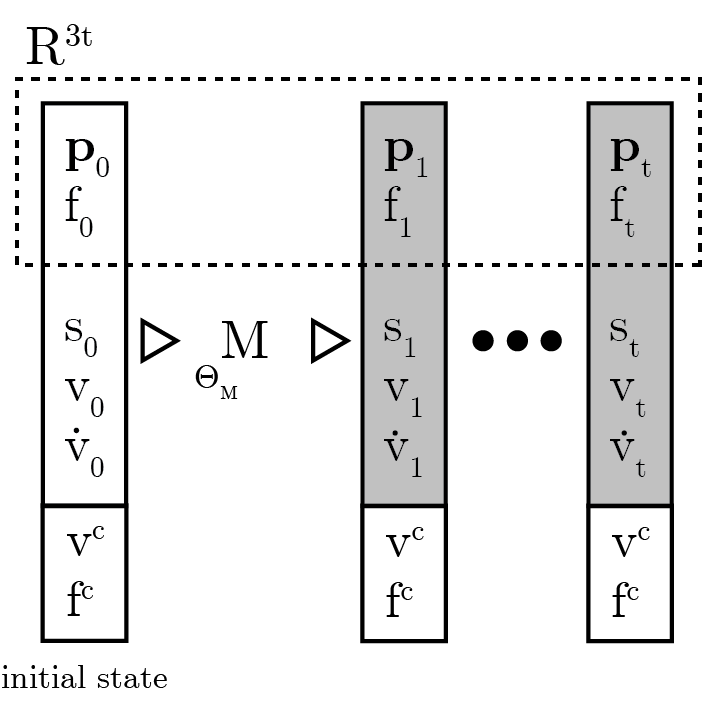
\includegraphics[width=0.5\columnwidth]{img/model_flow.png}
    \caption{Movement Model update computation for generating the evaluation space. White and grey background indicate values in the Control Genome and generated by the Movement Model respectively. \kenny{Observe the recursive forward evaluation nature in the update.}}
    \label{fig:control:modelflow}
\end{figure}

An analytical model like this can be of great practical use to the game developers. The parameters have direct links to explainable properties in the animation which makes it easier to tweak the behavior of the model. On the other hand, the analytical approach requires that the designers are able to adequately model the complexity of the movement. 
%
\kenny{The next sentence fells out of place? Are you talking about what people are doing or what we want to do?}
When this is not the case, we can apply machine learning techniques to discover latent properties of our animation set. % 
One approach is to extract a limited latent variable set using a dense neural network and then feed the latent variables to a set a primitives which are weighted to give the final output. 
Alternatively, we could apply a hybrid approach by discovering correlations in the data by automated statistical analysis, but still allow the designer to setup the primitives and chose which parameters should be used. 
\kenny{If what was described above is current practice then I am missing some citations for it as well as some arguments/descriptions of why it is not clever and why what we are doing is better?}

Finally we note that multiple local Movement Models can be easily combined. Transitions between models can be established using the same primitives. In practice we find it is often sufficient to use a single 1D blend \kenny{This statement/section may promise an experiment to prove it}. For instance the shift between 'run' and 'walk', which could require individual models, is usually distinct and of limited complexity and duration. 

\subsection{Motion Alignment}
To fit a Movement Model and Control Genome pair we project reference animations to evaluation space by constructing $\edit$ as a 2 step function where $\trajest$:\textit{Trajectory Estimation} is followed by $\driftcor$:\textit{Drift Correction}. Using similar convention as in the previous section we map animations of $t$ frames to evaluation space. 
\kenny{$\anim_{t}^{\dimas}$ is used in $\edit$ but $\trajest$ takes only $\anim_{t}$ why is there not a superscript? or should superscript be removed all together?}
\begin{subequations}
\begin{align}
    \edit(\parame,\anim_{t}^{\dimas})&:\driftcor(\parame,\trajest(\anim_t)) \,,\\
    \trajest&:R^{\dimas\times{t}} \rightarrow  R^{3t} \,,\\
    \driftcor&:R^{3t} \rightarrow R^{3t} \,.
\end{align}
\end{subequations}
Notice that only $\driftcor$ is parameterized.


Even simple animations contain details that makes it difficult to extract a reduced Control Genome. A recording of a straight walk does not contain a straight line in the bone movements of the subject. Projection of the hip bone or center of mass to the ground plane has cyclical components due to the nature of human locomotion. Additionally, the subject might drift on and off the instructed straight path. We need complex Control Genomes to model such details. 
Informally $\edit$ extracts an idealized movement path from animations by removing noise and applying slight corrections. Ie. a straight walk is estimated as a sequence of local line segments, which are then corrected to produce a single straight trajectory. The animation can now be described by a further reduced Control Genome of just a single direction.

\subsubsection{\bf Trajectory Estimation}
\magnus{If two consecutive steps are with same foot, we insert at 'fake' step to keep ping-pong}
It is common to extract trajectories by filtering bone positions and projecting to the ground plane. Usually a temporal smoothing is applied to either the hip [ref] or an estimated center of mass [ref]. In some cases the filter is made context aware to prevent masking of low frequency details in turning movements. We propose an alternative approach where foot contacts are used as guiding points. Given that environment contacts is used to change movement direction, it seems natural that trajectory information can be extracted from contact analysis. We show that this approach yields trajectories that are more stable and corresponds better to intuitively observable trajectory of an animation than what is produced by bone filtering \magnus{Also required no tuning of a smoothing filter}\kenny{Make sure we have experiments to prove claims and compare contact-trajectories to filtering trajectories. It would be nice to make figure references here, as seen in Figure XX}.
%
Although similar techniques have been described before [ref] we have not seen the approach used for trajectory estimation.
Contacts are detected using a height/velocity heuristic for the foot bones. A preliminary line is traced by connecting center point between adjacent right-left foot contact pairs. At each contact point we locate synchronization points on the preliminary line that is closest to hip bone position at the corresponding time. Trajectory samples are evenly spaced between synchronization points at a rate controlled by animation frame distances between the associated hip positions. The process is illustrated in Fig. \ref{fig:method:trajectory}. 
\begin{figure}
    \centering
    \kenny{This figure is conceptually nice. I think it is worthwhile to keep in. However, if the rendering style could look more like the one in Fig 8, so style are more coherent, then that would be great.\\}
    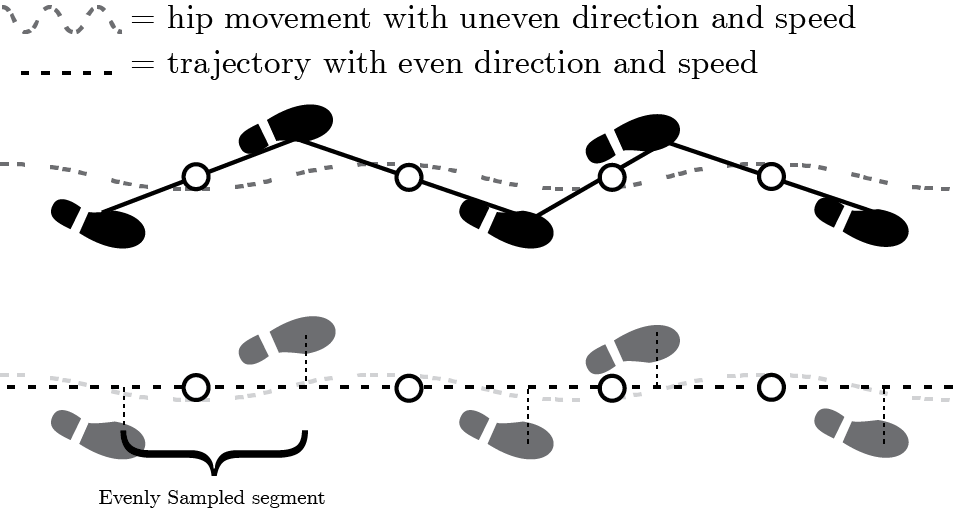
\includegraphics[width=1\columnwidth]{img/trajectory.png}
    \caption{Trajectory estimation from center of feet positions. Observe how the mid-points between feet center points generate a more straight trajectory compared to the filtered root motion that oscillates.}
    \label{fig:method:trajectory}
\end{figure}

\subsubsection{\bf Drift Correction} 
We apply adjustment curves by distributing $\parame,$ adjustment keyframes along the trajectory. With high $\counte$-values \kenny{It is not clear what $\counte$ is? } adjustment values change frequently due to the higher number of key frames. By decreasing $\counte$ we achieve smoother adjustment. Each keyframe is associated with a rotation and per frame values are interpolated along the curve to ensure smooth changes. The adjustment curve is applied by accumulating rotations along the entire animation, so that an adjustment rotation at frame $n$ influences all frames $>n$. An example in shown in Fig. \ref{fig:method:adjustment}. 

Adjustment curves can align evaluation space vectors (trajectories) $v_0,v_1\in R^{3t}$ by an optimization
\begin{subequations}
\begin{align}
    \arg\min_{\parame}{
        \frac{1}{2}|v_0-\driftcor(\parame,v_1)|^2
    }
\end{align}
\end{subequations}
We apply such an alignment as a post processing step in the optimization procedure. In this case adjustments keyframes are distributed at 2Hz. 

For Drift Correction we optimize to fit $v \in R^{3t}$ against a linear least squares fit. \kenny{Is optimization not wrt to $v$? I think I am little confused, because I see two optimization problems? I think maybe you should just drop the first version?}
\begin{subequations}
\begin{align}
    \arg\min_{\parame}{
        \frac{1}{2}|\mathcal{LLS}(v)-\driftcor(\omega\,\parame,v_1)|^2
    }
\end{align}
\end{subequations}
We apply the procedure to local segments of the animation that are almost straight. Straight segments are identified as regions between neighboring Control Genome changes, where $\omega$ is a weight vector used to disable alignment close to the local end points. In this case the keyframes are distributed only at 1Hz. The heuristic works well for animations consisting of turns and straight segments, but it is quite brittle and needs careful animation dependent tuning of the weights to avoid unwanted straightening of curved sections.
\begin{figure}
    \centering
    \kenny{I dislike the style of the figure. It stands out compared to the better visual quality papers. A coherent style everywhere is better, if style looks messy then it colors reviewers opinion of the work.\\}
    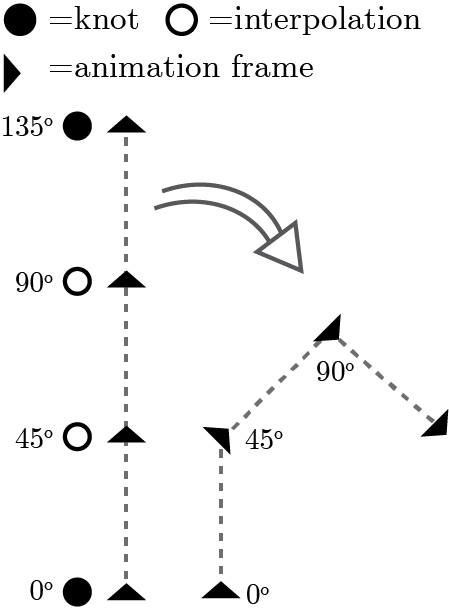
\includegraphics[width=0.5\columnwidth]{img/adjustmentcurve.png}
    \caption{Adjustment Curve}
    \label{fig:method:adjustment}
\end{figure}

\subsection{Optimization}
We use a multi step optimization consisting of three independent passes. The procedure takes a reference animation and a Movement Model as input. Control Genomes are annotated by hand or generated automatically. We use the latter approach. Parameters are fitted locally to each Control Genome and associated animation segments in S. The locally fitted models are combined in a final pass. The Control Genome granularity can be increased if the combined model exhibits poor behavior.
\begin{itemize}
    \item {\bf{Step 1: Trajectory Estimation \& LLS Alignment}} is applied to the input animation. The output is an evaluation space vector. Control Genomes are generated from the vector using a heuristic where entries are added when the vector tangent changes above a threshold. The input animation is updated to use the estimated trajectory.\magnus{Maybe figure ?}\kenny{Yes, please}
    \item {\bf{Step 2: Movement model fitting}} optimizes the parameters of the Movement Model and Control Genome adjustments to fit the generated evaluation space vector. Control Genomes are adjusted to allow wiggle room in the timings and directions.
    \item {\bf{Step 3: Model combination \& Post Alignment}} uses adjustment curves to fit the reference animation to movement produced by the combined Movemement Model. Depending on the density of adjustment keyframes this step decreases animation quality. The sum of adjustment keyframes values can be used as an indicator for the accuracy of the previous fitting. We find that metrics for evaluation of animation quality are hard to establish, and refer to the accompanying video for assessment of fit quality as a supplement to error plots.
\end{itemize}


\begin{algorithm}
    \SetAlgoLined
    \KwIn{$A$: Reference animations, $M$: Movement Model}
    $\theta^{*}_{M} \leftarrow$ initialize global model parameters\\
    $T\in R^{3t} \leftarrow \{A\}$, estimate trajectory\\
    $S \leftarrow \{T\}$, extract genome/segment map\\
    \ForEach{$\{G,seg\} \in S$} {
        $\theta_{M} \leftarrow$ initialize local model parameters\\
        $\theta_{G} \leftarrow$ initialize Genome adjustments\\
        $\nabla{\theta} \leftarrow \nabla{\theta_{seg}},\nabla{\theta_{G}}$, initialize gradients\\
        $optim \leftarrow$ initialize optimizer\\
        $T_{seg} \leftarrow \{T,seg\}$, get animation segment\\
        $T_{\edit} \leftarrow \{G,T_{seg}\}$, apply drift correction\\
        \For{optimizer steps}{
            $T_M \leftarrow \{M,G,\theta_{seg}\}$, unroll Movement Model\\
            $loss \leftarrow \{T_M,T_{seg}\}$, MSELoss of modeled movement\\
            \For{$\nabla\theta_i != 0 \in \nabla\theta$} {
                $loss += \{\theta_i\}$, add L2 regularization\\
            }
            $\nabla\theta \leftarrow loss$, backtrack\\
            $\theta_M,\theta_G \leftarrow \nabla\theta$, gradient descent\\
        }
        $S \leftarrow \{\theta_G\}$, store genome adjustments\\
        $\theta^{*}_{M} \leftarrow \{\theta_G$\}, store model parameters
    }
    $A \leftarrow \{M,G \in S,\theta^{*}_{M}\}$, align full animation to model fit 
    \caption{Fitting Procedure}\label{algo:optim}
    \end{algorithm}
 We use PyTorch auto differentiation with gradient descent for the implementation. The procedure is shown in Algorithm. \ref{algo:optim}. Good convergence requires continuous gradients across the parameter space. We use branchless programming techniques and PyTorch constructs for non-continuous functions. In the implementation of movement primitives, absolute() is used to guard against negative parameters, and GreaterThan/LessThan() for branchless if statements. While discontinuities are introduced, we find that the optimization is still able to arrive at expected minima, probably because the discontinuities lie between unrelated areas of the parameter space.

To use a global learning rate for the optimizer, we normalize the range of all parameters and apply fixed constant scalings. This is easily doable since most parameters have direct physical counter parts such as velocity, turn angles etc. Scale values can then be identified by doing a pre-pass over the animation. This in turn limits the impact of local minima, as the optimization can be given plausible initialization values.

L2 parameter regularization is applied to avoid interpolations between extreme parameter values within the movement primitives, which can be difficult to interpret and modify for a human. Parameters with zero gradients are not activated by the reference animation, and regularization is disabled to avoid loss decrease as a result of decreasing unused parameters.

